\subsection{Магнитометър}


Изпозван е чип \textit{LIS3MDL} (\autoref{fig:mag_directions_and_pinout}) \cite{magnetometerrefman},
който е интегрирано пакетно решение, 
предоставящо магнитометър по 3 оси.
Чипът използва \(1.9 \to 3.6V\) захранване катo в нужния решим  консумира  не повече от \(270\mu A\).
Чипът е част от сензорна платка, позволяваща директна връзка чрез протокол \textit{I2C} (адрес: \texttt{0x3C}).

За целите на настоящия проект е използвана следната конфигурация:
директен достъп (без буфериране) до измерените стойности;
обхват на всички оси \(\pm 8gaus\).


\begin{figure}[htpb!]
    \centering
    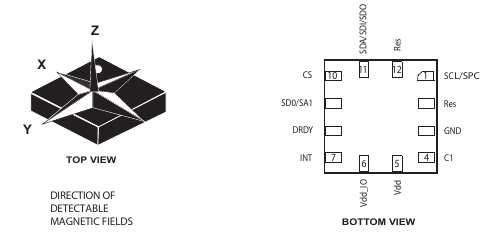
\includegraphics[width=0.7\textwidth]{mag_directions_and_pinout}
    \caption{Магнитометър -- оси на измерване и наименования на пиновете}
    \label{fig:mag_directions_and_pinout}
\end{figure}

\FloatBarrier
